%% METHOD SECTION %%

\section{Method}

%This section describes the research methodologies used for data collection and data analysis. Additionally, it presents the characteristics of the papers in our reviewed corpus.

\subsection{Data Collection}
To perform a literature analysis of past findings on the relationship between the specifics of conversation architecture and perceptions of CAs, we identified, reviewed, and selected relevant literature using PRISMA guidelines \cite{prisma}. %, we reviewed and selected literature exploring the relationship between the specifics of conversation architecture elements and perceptions of CAs. 
Searches were carried out in the ACM Digital Library between January 1 and January 15, 2023. Through our analysis, we didn't find any common terms used to refer to either conversation architecture elements or aspects of perceptions. As such, we generalized our search term to capture articles related to conversational agents. Based on search terms used in previously published literature reviews \cite{clark2019state, rapp2021human}, the following keywords are used to search for publications related to conversational user interfaces:
\newline

\textit{"conversational agent" OR "natural language interface" OR "IPA" OR "intelligent personal assistant" OR "chatbot" OR "speech interface" OR "voice assistant" OR "intelligent agent" OR "human-chatbot communication" OR "virtual agent" OR "dialog* system" OR "voice user interface" OR "human computer dialog*"}
\newline

The following selection criteria are applied to identify literature related to the effect of conversational architecture on the perception of agents:
\begin{itemize}
  \item The paper was published between 2010 and 2022.
  \item The paper is peer-reviewed and written in English.
  \item The paper contains the use of voice-based or text-based conversational agents.
  \item The paper contains studies on the impact of conversation architecture elements on the perceptions of agents.
  \item The paper contains impact of conversation architecture elements can be separated from other effects (e.g. embodiment).

\end{itemize}

The initial query retrieved 2901 unique publications. We screened the titles and abstracts of the papers based on the selection criteria above, resulting in 221 papers. The fully body of these papers were then reviewed, selecting 49 papers that met the criteria. A search for additional literature based on citation tracing was also performed to supplement the corpus, adding 8 more papers to the selection. In total, we identified 57 relevant articles for analysis (see \autoref{fig:prisma}).

%% PRISMA Process Visualization %%

\begin{figure}[h]
  \centering
  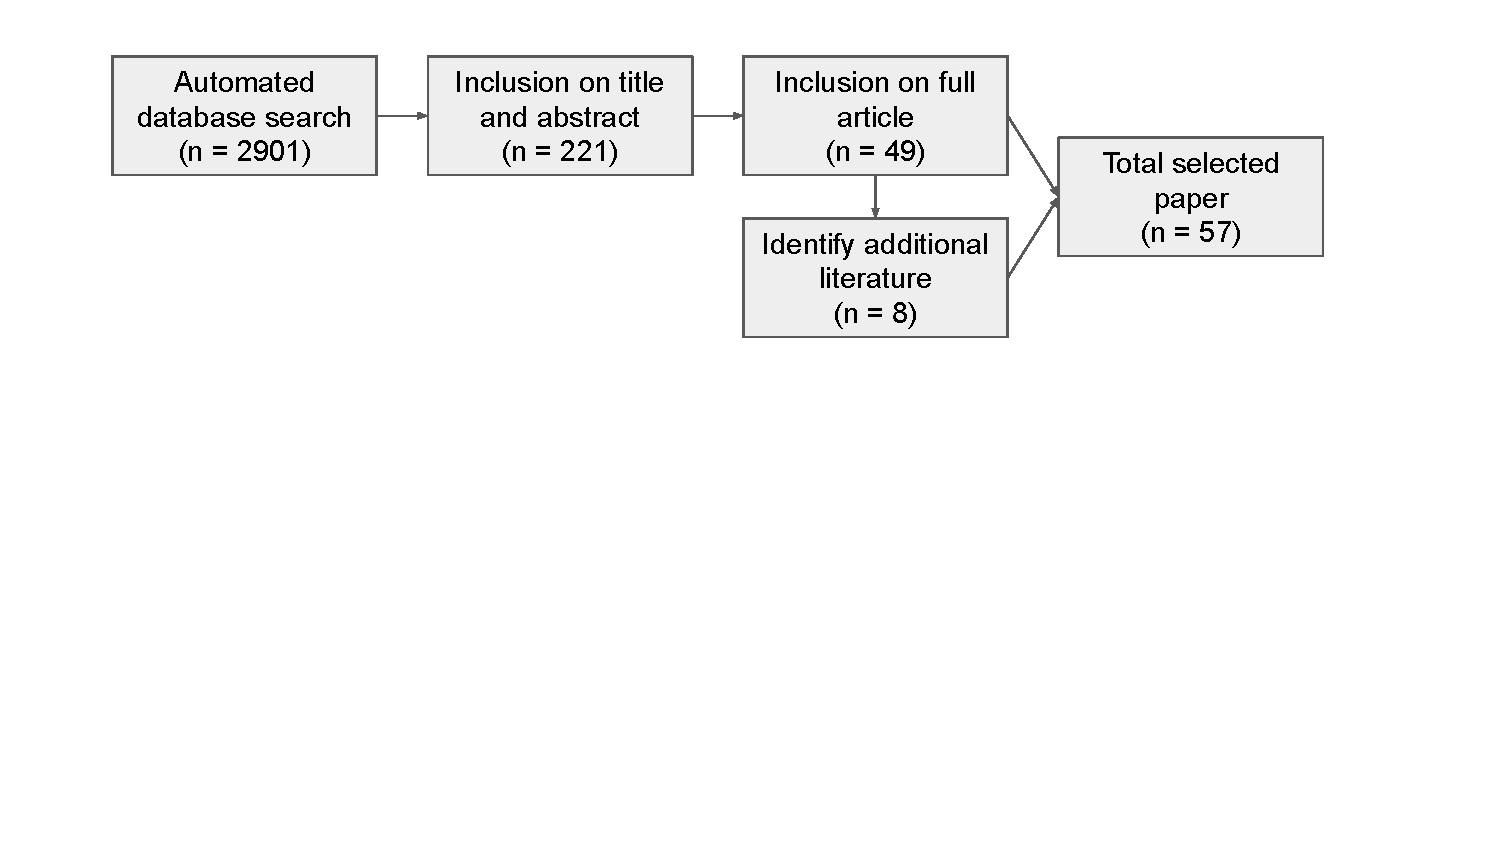
\includegraphics[width=1\columnwidth]{figures/fig-prisma.pdf}
  \caption{Literature search using PRISMA guidelines}
  \label{fig:prisma}
\end{figure}

\subsubsection*{Literature Corpus Characteristics}

The papers reviewed (n=57) were published between May 2011 and November 2022. The majority of the papers were published in or after 2019, with a slight trend upwards over the years (see \autoref{fig:paper}). The vast majority of the papers in our corpus were published in conference proceedings (n=50), with the remainder papers published in journals. Out of the papers published in conferences, the top conferences were The ACM Conference on Human Factors in Computing Systems\footnote{https://dl.acm.org/conference/chi} (n=16), Conversational User Interfaces\footnote{https://dl.acm.org/conference/cui} (n=7), Human-Agent Interaction\footnote{https://dl.acm.org/conference/hai} (n=4), and Intelligent Virtual Agents\footnote{https://dl.acm.org/conference/iva} (n=4). 
%Out of the papers published in journals, some venues include the International Journal of Human-Computer Interaction\footnote{https://www.tandfonline.com/journals/hihc20} (n=2) and Interacting with Computers\footnote{https://academic.oup.com/iwc} (n=1).

On the modality characteristics of the conversational agents in the corpus, there is a roughly even split between the modalities, with slightly more papers exploring voice-based CAs (n=30) compared to text-based CAs (n=27).

%% Number of papers by year figure %%

\begin{figure}[h]
  \centering
  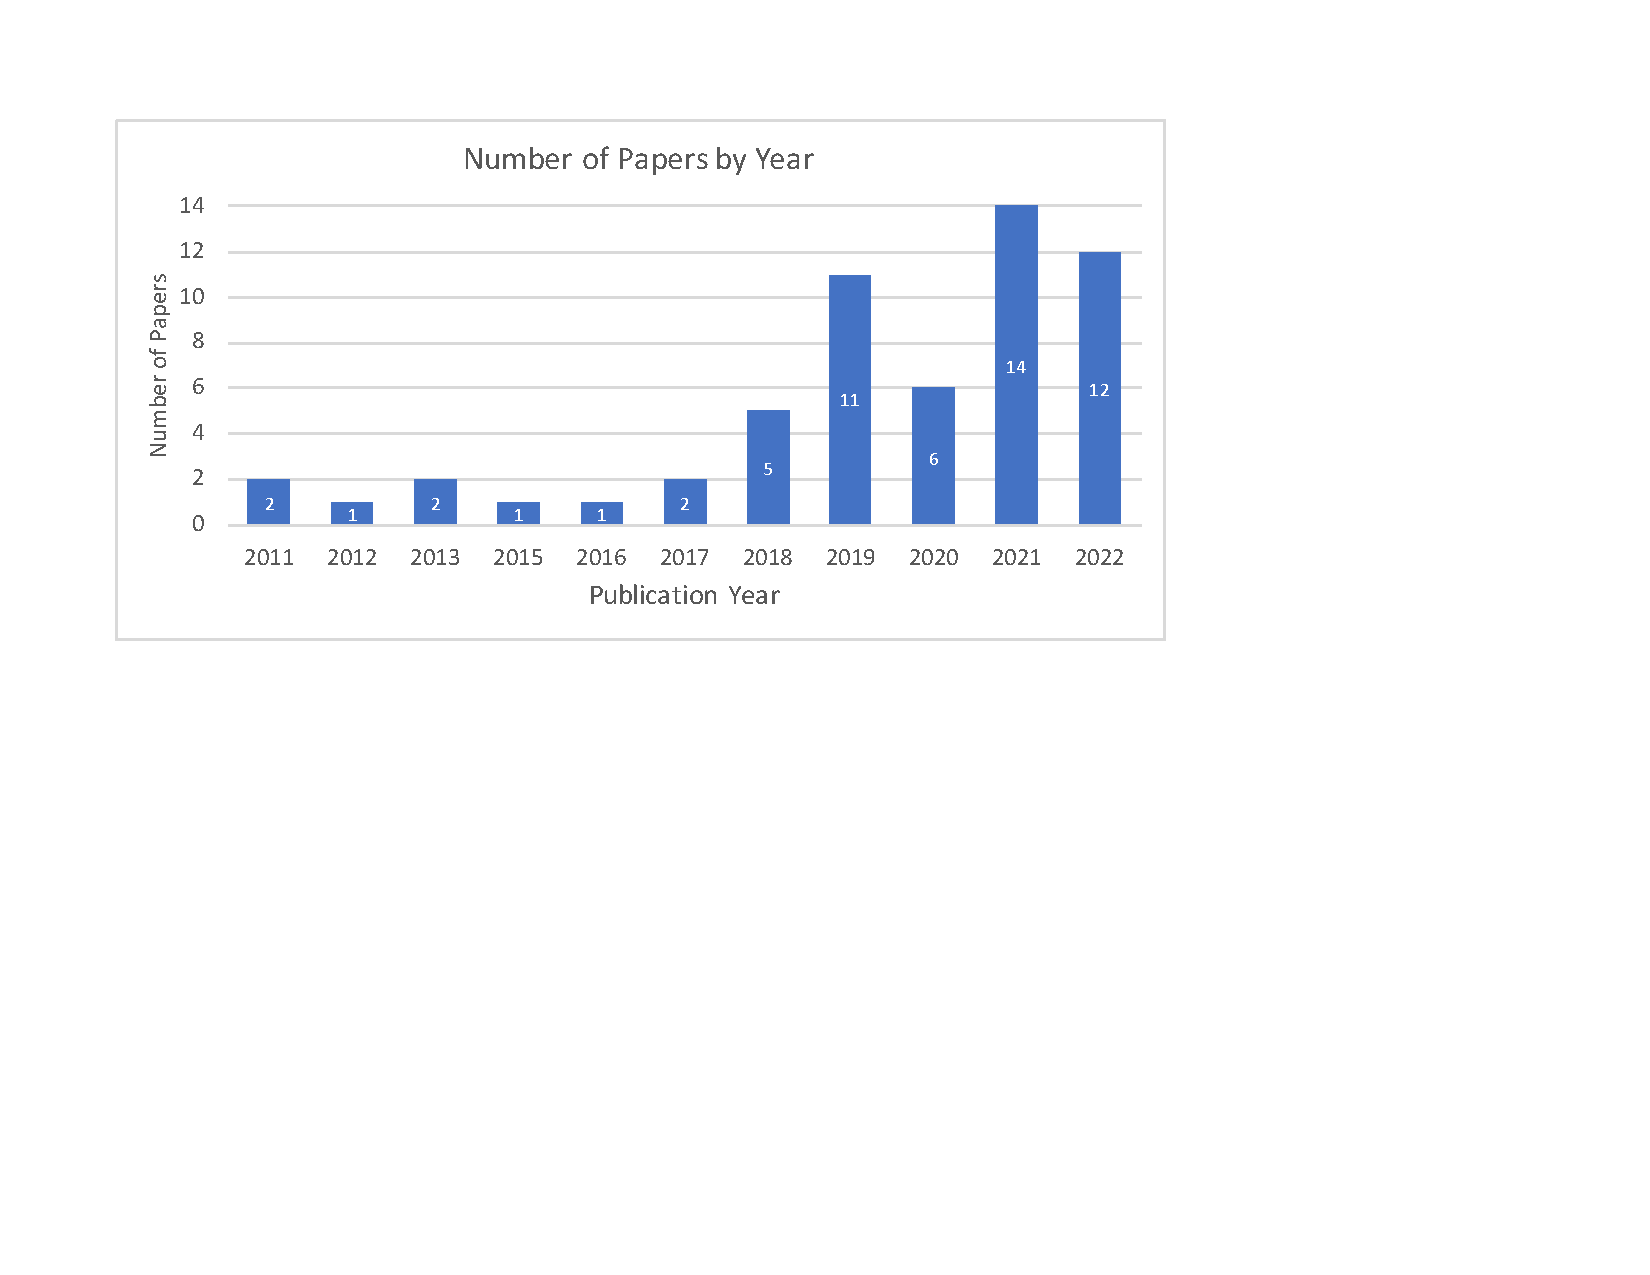
\includegraphics[width=\columnwidth]{figures/fig-paper.pdf}
  \caption{Number of papers by year}
  \Description{This graph shows the number of publications by year in our reviewed corpus between 2011 to 2022. There is a small number of papers each year between 2011 to 2017, with more papers per year starting in 2018. There is an upward trend on the number of publications over the years.}
  \label{fig:paper}
\end{figure}

\subsection{Data Analysis}

\subsubsection*{Perceptions of Agents} To understand the perceptions of agents related to conversation architecture (RQ1), assessments for the perceptions of agents were extracted from each paper. We used inductive thematic analysis to group these assessments into codes based on their meanings. For example, the code likeability of the agent contains the questionnaire item "this voice agent was likeable" used by \cite{cuadra2021my}\cmt{[67]}, Godspeed questionnaire \cite{bartneck2009measurement}\cmt{godspeed}'s set of questions on likeability used by \cite{linnemann2018can}\cmt{[15]}, and Subjective Assessment of Speech System Interface (SASSI) questionnaire \cite{hone2000towards}\cmt{sassi}'s set of questions on likeability used by \cite{chan2021kinvoices, choi2020nobody}\cmt{[74][54]}. This step resulted in 83 unique codes. These codes are then organized based on similarity of the meanings, resulting in 11 aspects of perceptions. For example, the aspect of personality traits of the agent contains measurements such as likeability, funniness, and kindness. Lastly, the 11 aspects are grouped into 4 categories: perception of interaction with agent, perception of agent's ability, perception of sociability with agent, and perception of agent's humanness (\autoref{tbl:perceptions}).

\subsubsection*{Conversation Architecture Elements}
As to the elements of conversation architecture that are relevant to the perception of agents (RQ2), we extracted the specifics of conversation architecture used in each paper. Some of the papers used multiple features in their CA design, such as the the anthropomorphic agent used in Seeger et al's study \cite{seeger2021chatbots}\cmt{[35]}. In these composite situations, we broke them down into their individual features. For example, the anthropomorphic agent \cite{seeger2021chatbots}\cmt{[35]} was separated into emotional expressions, is-typing indicator, emoticons, and response delay and captured as codes. 58 unique codes were created as part of this process, capturing features like sentiment-adaptive responses \cite{diederich2019emulating}\cmt{[25]}, lexical alignment \cite{spillner2021talk}\cmt{[18]}, and typos \cite{westerman2019believe}\cmt{[9]}. We then organized these codes into elements based on similarity, resulting in 12 elements of conversation architecture. For example, the element of disfluency contains fillers \cite{jeong2019exploring, wester2015artificial}\cmt{[10][14]}, interjections \cite{ceha2022expressive, hu2021enhancing}\cmt{[77][56]}, repetitions \cite{yang2021effect}\cmt{[72]} and typos \cite{westerman2019believe}\cmt{[9]}. These elements are grouped into 4 categories: dialog strategy, content affectiveness, content style, and speech format (\autoref{tbl:conversation_architecture}).

\subsubsection*{Relationship Between Perceptions of Agents and Conversation Architecture}

%% Heatmap of the identified relationships between perceptions & conversation architecture

\begin{figure*}[]
  \centering
  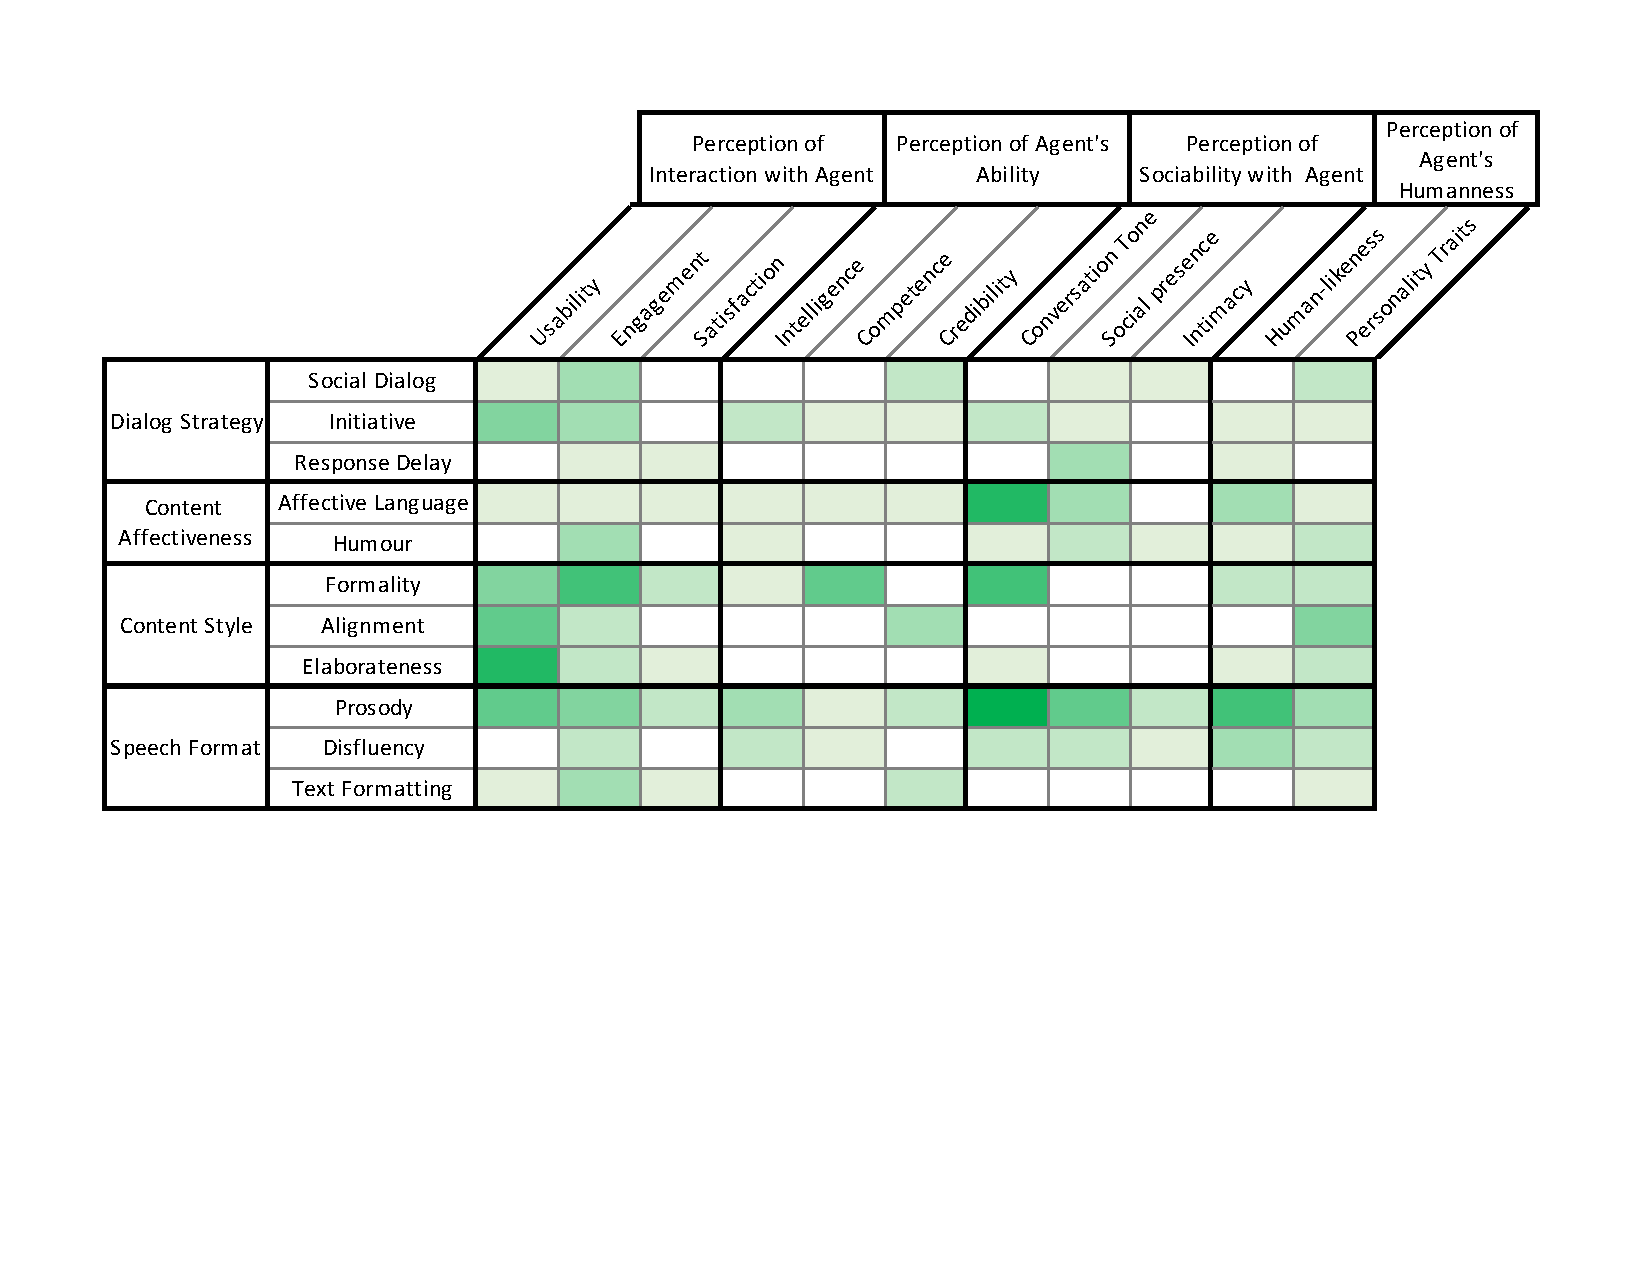
\includegraphics[width=\textwidth]{figures/fig-heatmap_identified.pdf}
  \caption{Heatmap of literature for perception of conversational agents for each type of conversational architecture element}
  \label{fig:heatmap_identified}
\end{figure*}

To study the effect of conversation architecture on users' perceptions (RQ3), we extracted the connections explored in each paper, using the perception aspects and conversation architecture elements developed in the previous data analysis steps. Each connection's effect was also recorded based on whether an association was found in the study and the nature of that association. Out of our review corpus, 265 connections between perceptions of agents and conversation architecture were explored in literature. To analyze the specifics of conversation architecture that affect the perceptions of CAs, 72 connections that did not result in observed relationships were discarded, resulting in 193 relationships for analysis. For example, the connection between the matching style of a CA and user satisfaction was removed because Hoegen et al. \cite{hoegen2019end}\cmt{[31]} did not find a significant difference between the style matching agent and the non-style matching agent for overall interaction satisfaction. Out of the 193 relationships, 10 were relationships based on agents modifying multiple architecture elements (e.g. \cite{seeger2021chatbots, volkel2021manipulating}\cmt{[35][68]}). They were not included in the final framework as we could not attribute the perceptions of agents to the underlying core elements. Overall, 183 relationships between individual architecture elements and perceptions of agents are incorporated into our synthesized framework, visualized as a heatmap to demonstrate their relationships with each other (\autoref{fig:heatmap_identified}).